%%%%%%%%%%%%%%%%%%%%%%%%%%%%%%%%%%%%%%%%%%%%%%%%%%%%%%%%%%%%%%%%%%%%%%%%
% Visual Analytics of Bitcoin: A Multi-Scale Dashboard for Market
% Regime Discovery and Event Explanation
%
% MSBD5005 — Data Visualization (Spring 2026)
% Team USTVIS14 (Team 14): CAI, HUANG, LU, ZHANG, ZHANG
%
% Built against the IEEE VGTC conference template.  See report/README.md
% for the one-time setup (drop `vgtc.cls` + the bundled .bst into this
% folder, then `latexmk -pdf main.tex`).
%%%%%%%%%%%%%%%%%%%%%%%%%%%%%%%%%%%%%%%%%%%%%%%%%%%%%%%%%%%%%%%%%%%%%%%%

\documentclass[journal]{vgtc}                  % VGTC journal/conference style
% Fallback for environments without vgtc.cls — uncomment to draft in plain
% LaTeX before the VGTC class is installed.  The two-column geometry below
% mimics the VGTC look closely enough for word-count and layout review.
%
% \documentclass[10pt,twocolumn,letterpaper]{article}
% \usepackage[margin=0.75in]{geometry}
% \usepackage{times}

\usepackage{graphicx}
\usepackage{times}
\usepackage{amsmath}
\usepackage{amssymb}
\usepackage{xcolor}
\usepackage{hyperref}
\usepackage{booktabs}
\usepackage{microtype}

\hypersetup{
  colorlinks=true,
  linkcolor=black,
  citecolor=black,
  urlcolor=blue!50!black,
}

%% Paper title.
\title{Visual Analytics of Bitcoin:\\A Multi-Scale Dashboard for Market Regime
Discovery and Event Explanation}

%% Author block.  The VGTC class wraps these into the standard header.
\author{Zhuoang Cai\thanks{e-mail: zhuoangc@outlook.com}
\and Jiaxin Huang
\and Wanlin Lu
\and Jialin Zhang
\and Xiaotong Zhang}
\affiliation{\scshape Hong Kong University of Science and Technology
\textperiodcentered{} MSBD5005 Spring 2026}

%% Teaser image (optional).  Uncomment when a hero figure is available.
% \teaser{
%   \includegraphics[width=\linewidth]{figures/teaser.png}
%   \caption{The three coordinated views during the 2026-03-23 Iran-tension
%   case study.  Brushing the Macro window propagates to Meso and Micro;
%   the headline panel and Polymarket panel surface the day's narrative.}
% }

\abstract{%
A price chart shows that Bitcoin moved.  It cannot show \emph{when}, \emph{what
kind of day}, or \emph{why}.  We present a coordinated multi-scale dashboard
that answers all three across one interaction loop: a \textbf{Macro} long-range
overview, a \textbf{Meso} regime-discovery view built on a UMAP projection of
eight engineered daily features, and a \textbf{Micro} day-explanation view
that pairs intraday price action with same-day GDELT headlines and Polymarket
prediction-market odds.  The three views share a single Zustand store, so a
brush in one filters the others.  Beyond the chart inventory, the system makes
a small but practical data-design contribution: per-window \emph{curated} GDELT
queries and Polymarket event slugs that turn the recency-biased public APIs
into a date-aware historical context engine for four case-study windows
(COVID 2020, War 2022, Election 2024, Iran 2026).  We validate the workflow on
2026-03-23 — an Iran-tension day with a midday Bitcoin breakout — tracing the
narrative end-to-end from Macro anomaly to headline timing and prediction
odds.%
}

\CCScatlist{
  \CCScat{K.6.1}{Management of Computing and Information Systems}%
                {Project and People Management}{Life Cycle};
  \CCScat{K.7.m}{The Computing Profession}{Miscellaneous}{Ethics}}

\teaser{}

\begin{document}

\maketitle

%% ===================================================================
\section{Introduction}
%% ===================================================================

Bitcoin (BTC) sits between an asset and a narrative.  Its price has tripled and
halved multiple times since 2019, with each regime change tied to a different
external story: a pandemic crash, a Federal Reserve pivot, a sovereign war,
two US elections, and a string of geopolitical shocks.  A line chart can show
the magnitude of those moves; it cannot tell the analyst \emph{when} a regime
began, \emph{what kind of trading day} sits inside that regime, or \emph{why}
the market interpreted a given news bundle the way it did.

This project builds a web-based visual analytics system over a 2,677-day BTC
record (2019-01-01 to 2026-04-30) that answers all three questions in a single
interaction loop.  The system is organized around four analytical tasks
distilled from the project requirements:

\begin{itemize}
  \item[\textbf{T1}] \emph{Market evolution.}  How does Bitcoin evolve over
    the seven-year horizon?
  \item[\textbf{T2}] \emph{Pattern discovery.}  Which trading days form
    typical regimes, and which are abnormal?
  \item[\textbf{T3}] \emph{Day-level explanation.}  For a chosen day, what
    happened hour by hour?
  \item[\textbf{T4}] \emph{Cross-market context.}  How do news flow,
    prediction markets, and external assets relate to BTC?
\end{itemize}

Each task is served by one of three coordinated views (Macro, Meso, Micro)
plus a context layer that overlays GDELT headlines, Polymarket prediction-
market odds, and three external assets (COIN, MSTR, QQQ).  The three views
share a single Zustand selection store: brushing a Macro range filters the
Meso scatterplot, clicking a Meso point sets the Micro selected date, and
selecting a date in Micro highlights it back in Macro and Meso.  All four
data layers feed the same daily-bucket index, making cross-view linking a
constant-time lookup.

The system was deliberately scoped \emph{narrow and deep}: rather than build a
broad terminal-style toolkit, we focus on three high-bandwidth views and a
case-study navigator that walks the user through four prepared windows.  Our
case study below — 2026-03-23 — exercises every link in the chain.

%% ===================================================================
\section{Related Work}
%% ===================================================================

Our design draws on four threads of prior visualization work.

\paragraph{Coordinated multiple views and the overview-first pipeline.}
Munzner~\cite{munzner2014} formalizes the what/why/how triple that we use to
justify each chart: the Macro timeline is a position-on-common-scale derive,
the Meso scatterplot is a 2D-attribute summary, the Micro panel is a
time-aligned identity drill-down.  The Macro$\to$Meso$\to$Micro flow follows
Shneiderman's overview-first, zoom-and-filter, details-on-demand
mantra~\cite{shneiderman1996}.

\paragraph{Calendar heatmaps and time-series overviews.}
Van Wijk and van Selow~\cite{vanwijk1999} introduced the calendar-cell layout
we use to encode daily returns in Macro.  Heer and Bostock~\cite{heer2009}
documented the horizon-graph pattern for high-density time-series; we
considered it but reverted to a single-band timeline once event markers were
added, since the marker layer already supplies the vertical-density payoff.

\paragraph{Dimensionality reduction for daily market states.}
Each trading day is summarized by an eight-dimensional feature vector
(return, open-close change, high-low range, volume z-score, two rolling
volatilities, a 30-day drawdown, and a news-tone field).  We project to 2D
with UMAP~\cite{mcinnes2018umap} because, unlike PCA, it preserves both local
neighborhood and global cluster structure for non-linear feature mixes, and
unlike t-SNE it is reproducible across runs once a seed is fixed.  We then
overlay $k=5$ KMeans clusters with semantically calibrated labels (e.g.,
``Risk-Off,'' ``Bullish Momentum'').

\paragraph{Parallel coordinates and small-multiples summaries.}
Inselberg's parallel coordinates~\cite{inselberg1985} are the natural pairing
to a 2D embedding: they restore the original feature axes that UMAP collapsed.
Our cluster summary table follows the small-multiples idiom (Tufte's
``equity-curve sparklines'' applied to per-cluster cumulative returns).

\paragraph{News overlays in financial dashboards.}
Most public crypto dashboards (Glassnode, CoinGecko, TradingView) treat news
as a sidebar, decoupled from the chart.  Closer to our design intent are
ThemeRiver-style co-displays~\cite{havre2002themeriver} and prediction-market
overlays.  Our date-aware historical extension to GDELT and Polymarket — two
APIs that are structurally biased toward \emph{today} — is, to our knowledge,
the practical contribution that distinguishes this work from a chart catalog.

%% ===================================================================
\section{Design Tasks and Requirements}
%% ===================================================================

The four analytical tasks above translate into a small set of concrete design
requirements that shaped every chart choice:

\begin{description}
  \item[R1.\ Single-screen overview.]  All three views fit on a 1440-px
    laptop without scrolling for the active window.  This rules out heavy
    multi-tab terminals; it also forces information density choices (e.g.,
    sparklines instead of full charts where appropriate).
  \item[R2.\ Regime visibility.]  The Meso view must make the cluster
    membership of \emph{every} day in the brushed window legible at a glance.
    UMAP + colored hulls + a parallel-coords overlay collectively satisfy R2.
  \item[R3.\ Date-aware historical context.]  News and prediction-market
    panels must show what was true on the \emph{selected} date, not today.
    This is the requirement that drove the curated-bucket data design
    (Section~\ref{sec:system}).
  \item[R4.\ Brushing as causation control.]  Linking is bidirectional and
    constant-time: any selection propagates to all views in the same render
    cycle, so the user can hold a hypothesis (``March 23 looks anomalous'')
    and confirm or refute it across scales without breaking flow.
  \item[R5.\ Color-blind safety.]  Every diverging scale uses ColorBrewer
    RdYlGn-7; every categorical scale uses ColorBrewer Set2 with BTC orange
    excluded from cluster colors to avoid the BTC--cluster confusion.
  \item[R6.\ Bundle budget.]  $\le 6$~KB CSS gzip, $\le 130$~KB initial JS
    gzip; ECharts loaded lazily.  Current build: 5.00~KB CSS, 106.5~KB JS.
\end{description}

%% ===================================================================
\section{System and Visualization Design}
\label{sec:system}
%% ===================================================================

The system is a FastAPI backend serving three JSON endpoints
(\verb|/api/overview|, \verb|/api/meso|, \verb|/api/day-detail|) consumed by a
React 18 + Vite + Zustand frontend.  All visualizations are written in D3 v7
and ECharts v6; no chart library is used as a black box for our novel
encodings.

\subsection{Macro view (T1)}

The Macro view answers \emph{when}: it shows the BTC daily timeline together
with a calendar heatmap of daily returns, both bound to the same
\texttt{selectedTimeRange}.  The line uses position on a common scale —
Mackinlay's top-ranked channel for quantitative data~\cite{mackinlay1986} —
and is overlaid with five canonical event markers (FOMC pivots, war onsets,
ETF approvals).  The calendar heatmap uses ColorBrewer RdYlGn-7 anchored at
zero, so a single deep-red cell is the visual question that triggers a Micro
drill-down.  An event-density dot in the corner of each cell signals days
with $\geq 1$ GDELT article; the user can click any cell to set
\texttt{selectedDate}.

\subsection{Meso view (T2)}

The Meso view answers \emph{what kind of day}.  Its centerpiece is a UMAP
projection of the 8-dimensional daily feature vector to 2D, colored by
KMeans cluster with convex hulls drawn around each cluster's points.  The
cluster colors are deliberately Set2 (CB-safe) and explicitly exclude orange
to keep BTC's house color out of the categorical scale.

A \textbf{regime summary band} below the scatterplot makes the cluster story
quantitative:
\begin{itemize}
  \item A \textbf{cluster summary table} reports $n$, mean daily return,
    annualized volatility, and a 60-point \emph{equity-curve sparkline} for
    each cluster — small multiples (Tufte) so the reader compares regimes by
    \emph{shape}, not by scrolling between numbers.
  \item A \textbf{4$\times$4 cross-asset correlation matrix} (Pearson over the
    active window) over BTC, COIN, MSTR, and QQQ uses a diverging
    green$\leftrightarrow$red scale anchored at zero.
\end{itemize}

A toggleable \textbf{parallel-coordinates plot} over the seven engineered
features (Inselberg) restores the axes UMAP collapsed.  Selecting a cluster
in the legend filters all four panels in one render.

\subsection{Micro view (T3, T4)}

The Micro view answers \emph{what happened} on a selected day.  It is
composed of:

\begin{enumerate}
  \item \textbf{Summary cards} — selected-day open/high/low/close, intraday
    range, and 24-hour change with a redundant shape+hue $\blacktriangle/\blacktriangledown$ chip.
  \item \textbf{Intraday chart} — stacked OHLC candlesticks and volume bars
    sharing one x-axis, so position-on-common-scale carries the alignment.
  \item \textbf{External-asset context strip} — three small sparklines
    (COIN, MSTR, QQQ) over the same window, answering ``did everything else
    move with BTC?''
  \item \textbf{Headline panel (T4)} — GDELT articles for the selected day,
    sorted by tone, tagged with one of seven theme buckets (war, election,
    covid, regulation, macro, crypto, other).  The active GDELT
    \emph{bucket} (curated case-study window) is shown as a provenance line
    above the panel.
  \item \textbf{Polymarket panel (T4)} — per-curated-market cards each
    showing a daily YES-probability sparkline with a marker at the selected
    date, the YES price observed at that date, and the current resolution
    price.
\end{enumerate}

\subsection{Date-aware historical context: the data-design contribution}

The two public APIs we lean on for T4 are recency-biased.  GDELT's DOC API
returned bitcoin-only headlines for any query that matched
\verb|bitcoin OR crypto|, leaving COVID-2020 or election-2024 days with
near-empty headline panels.  Polymarket's keyword search returns
\emph{today's} active markets, useless for a query asking ``what did the
crowd believe on 2024-11-05.''

We solve both with the same \emph{curated-bucket} pattern.  Each of the four
case-study windows owns:

\begin{itemize}
  \item A tailored GDELT DOC query (e.g., the 2022 War bucket queries
    \verb|(ukraine OR russia OR putin OR sanctions OR swift OR ...)|) that
    keeps a \verb|bitcoin OR crypto| tail clause so the asset chart is
    always anchored, plus a six-category theme map (war, election, covid,
    regulation, macro, crypto) so non-crypto windows still produce a
    populated theme-tagged headline panel.
  \item A short list of curated Polymarket event slugs (e.g.,
    \verb|presidential-election-winner-2024|,
    \verb|us-iran-nuclear-deal-by-april-30|).  For each slug, we fetch the
    full Gamma event payload and the per-market CLOB \verb|/prices-history|
    daily series, then filter to markets active on the selected date with a
    14-day post-resolution grace window so the day-after-election market
    still surfaces with its closing probability.  A \$1k volume floor and
    top-8 cap drop the long tail of $\$0$ markets that would otherwise
    swamp the panel.
\end{itemize}

A bulk-warm script seeds 287 cached headline payloads and 6{,}700+
Polymarket price points across the four windows.  An auto-rollup step
re-emits \texttt{gdelt\_daily\_signals.csv} after every fetch so the Macro
heatmap dot-indicator stays in sync.  This is the piece that turns two
``today-only'' APIs into a date-aware historical context engine; it is
implemented in $\sim$300 lines of Python and is the contribution we are
proudest of beyond the chart inventory.

\begin{figure}[t]
  \centering
  \fbox{\rule{0pt}{40mm}\rule{0.95\linewidth}{0pt}}
  % 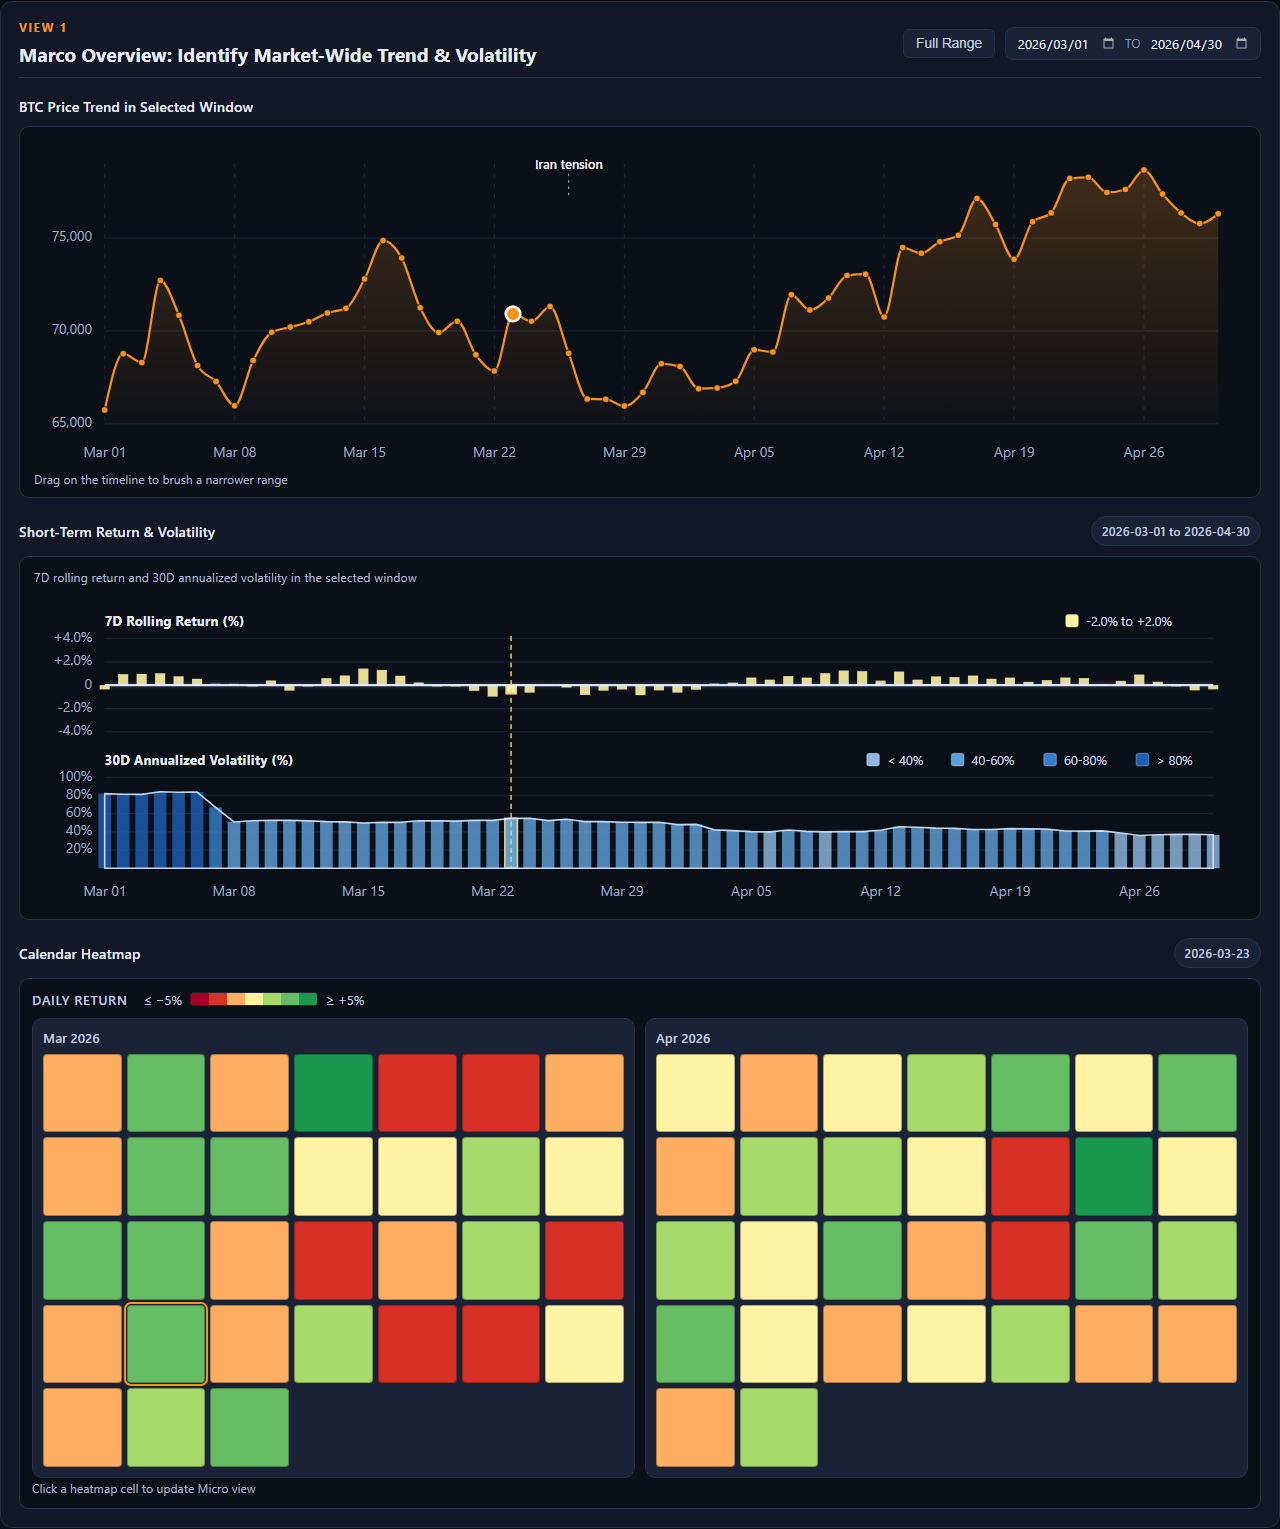
\includegraphics[width=\linewidth]{figures/macro.png}
  \caption{\textbf{Macro view (T1)} brushed to the 2026 Iran-tension window.
  Calendar-heatmap cells encode daily returns on a CB-safe diverging
  RdYlGn-7 scale anchored at zero; the deepest cell on 2026-03-23 is the
  visual question that drives the rest of the case study.  \emph{Figure
  placeholder; screenshot to be supplied by the team.}}
  \label{fig:macro}
\end{figure}

\begin{figure}[t]
  \centering
  \fbox{\rule{0pt}{40mm}\rule{0.95\linewidth}{0pt}}
  % 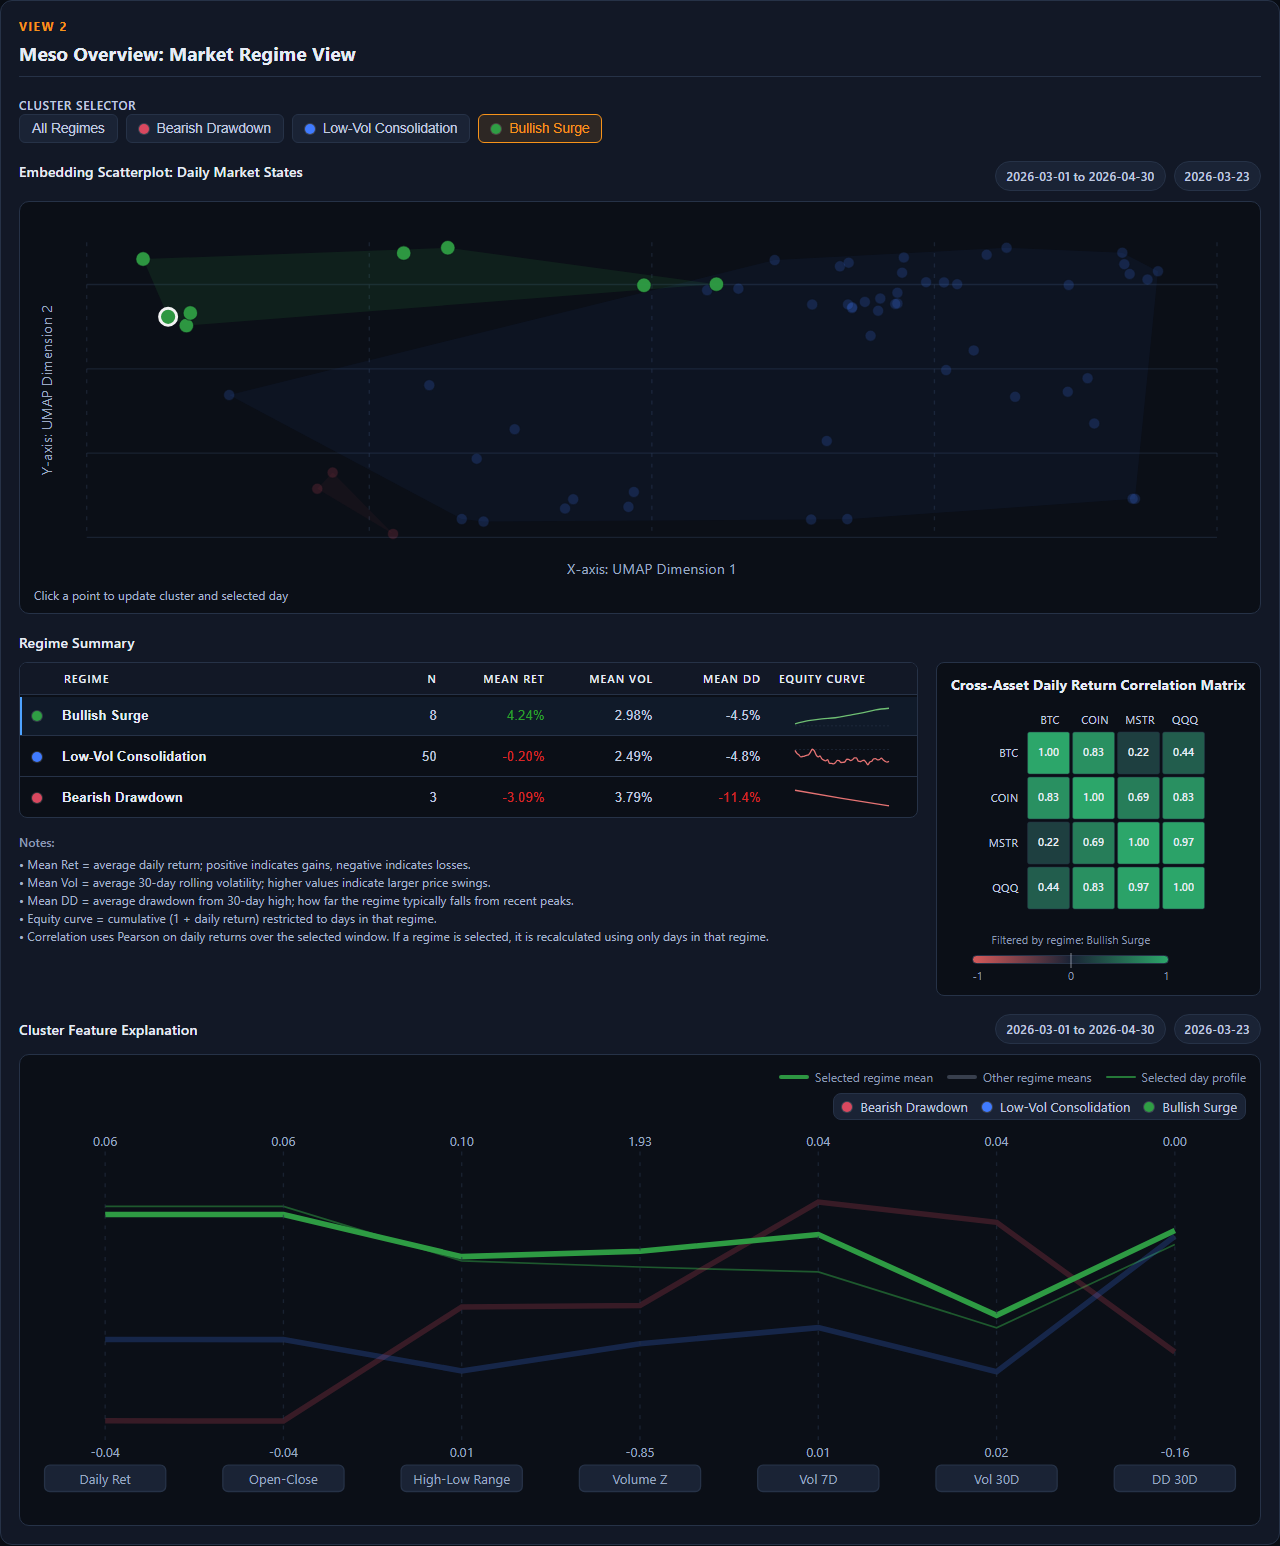
\includegraphics[width=\linewidth]{figures/meso.png}
  \caption{\textbf{Meso view (T2).}  UMAP projection of the 8-D daily
  feature vector colored by KMeans cluster, with convex hulls and the
  selected day (2026-03-23) marked.  The regime summary table (right) and
  parallel-coordinates plot (below, not shown) make the cluster
  characterization quantitative.  \emph{Placeholder.}}
  \label{fig:meso}
\end{figure}

\begin{figure}[t]
  \centering
  \fbox{\rule{0pt}{40mm}\rule{0.95\linewidth}{0pt}}
  % 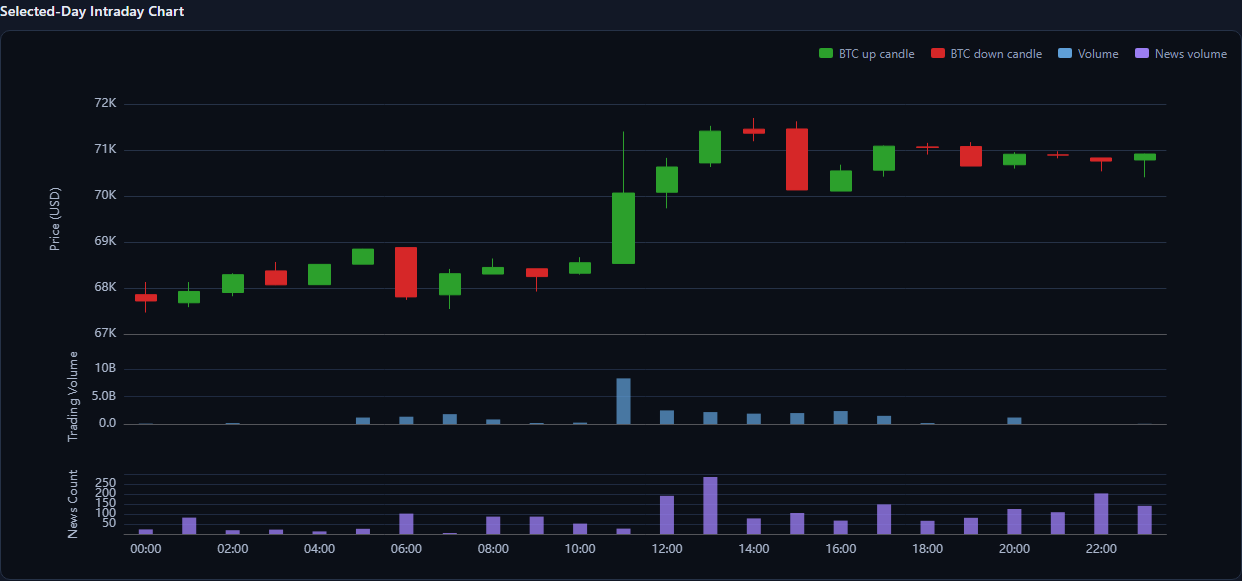
\includegraphics[width=\linewidth]{figures/micro-intraday.png}
  \caption{\textbf{Micro view: intraday OHLC + volume (T3)} for
  2026-03-23. The flat morning, midday breakout, and sustained afternoon
  rally are visible in three contiguous regimes; the volume bars confirm
  the breakout is not a thin-tape artifact.  \emph{Placeholder.}}
  \label{fig:micro-intraday}
\end{figure}

\begin{figure}[t]
  \centering
  \fbox{\rule{0pt}{40mm}\rule{0.95\linewidth}{0pt}}
  % 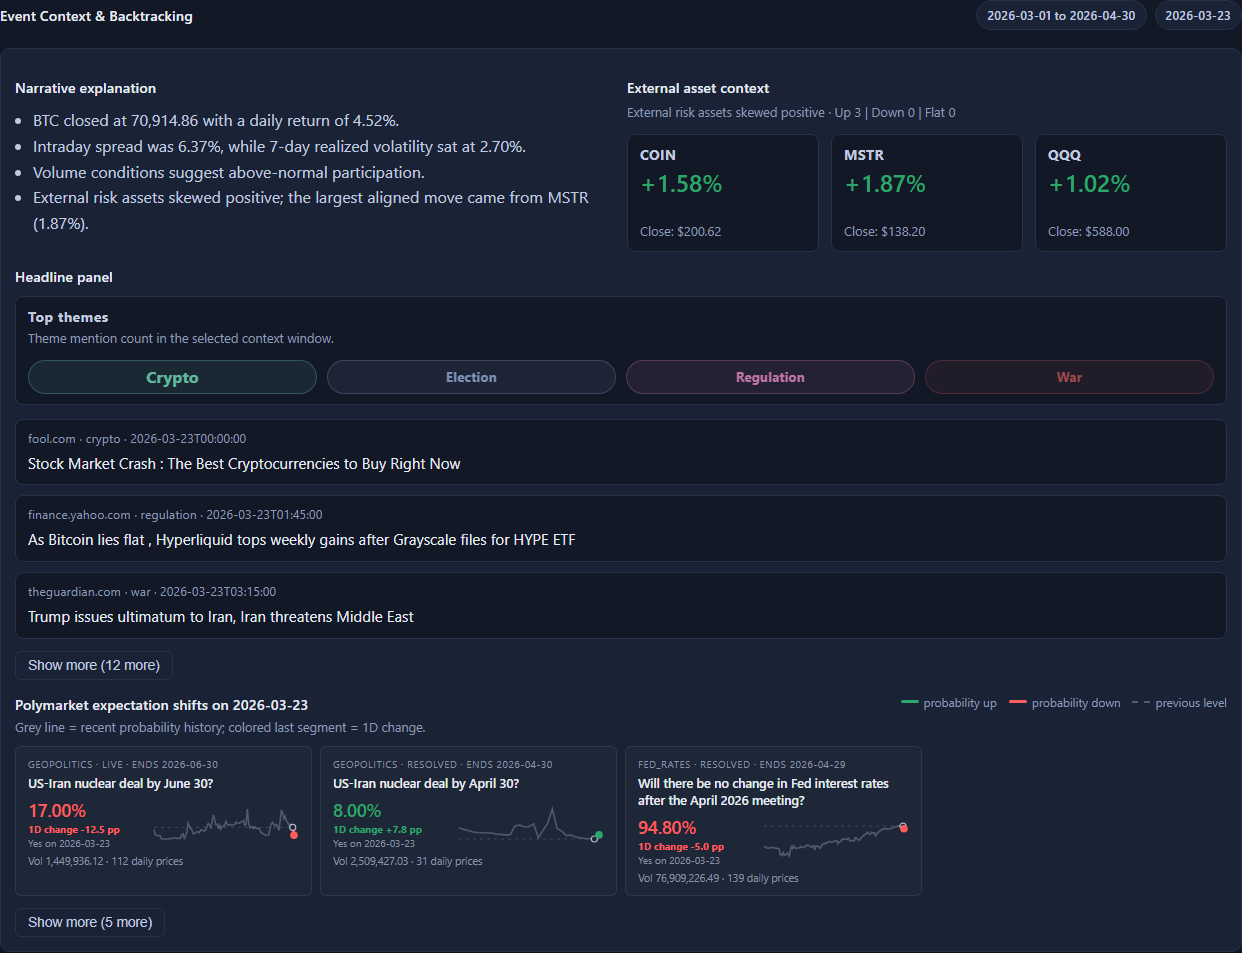
\includegraphics[width=\linewidth]{figures/micro-context.png}
  \caption{\textbf{Micro view: headline panel + Polymarket panel (T4).}
  Morning headlines lean negative and geopolitical; midday a concentration
  of mainstream price-breakout reports lands; afternoon shifts to mixed
  political/regulatory.  Polymarket cards show YES-probability sparklines
  with a marker at the selected date.  \emph{Placeholder.}}
  \label{fig:micro-context}
\end{figure}

%% ===================================================================
\section{Case Study: 2026-03-23, Iran Tension}
%% ===================================================================

We validate the workflow on a single deep case study — 2026-03-23, inside
the curated Iran-tension window.  The user begins from the case-study
navigator with no prior knowledge of the date.

\paragraph{T1 — locate the anomaly.}  The user clicks the \emph{Iran
Tension} chip.  The Macro window snaps to 2026-03-01 \(\to\) 2026-04-30.  In
the calendar heatmap (Fig.~\ref{fig:macro}), 2026-03-23 reads as a deep
green cell — a strong-positive day in an otherwise mixed window.  Hovering
shows the daily return; clicking sets \texttt{selectedDate}, which
propagates to Meso and Micro in the same render.

\paragraph{T2 — characterize the regime.}  In the Meso view
(Fig.~\ref{fig:meso}), the selected day lands inside the
\emph{Bullish-Momentum} cluster — the same cluster that contains other
midday-breakout days from the 2024 election cycle.  The parallel-coordinates
overlay shows that 2026-03-23's profile sits above the cluster mean on
\texttt{rolling\_volatility\_7d} and well below on
\texttt{drawdown\_from\_30d\_high} — the day is volatile but \emph{not}
correcting from a peak, which is consistent with a momentum breakout rather
than a relief rally.  The cluster summary table confirms this regime has
the steepest equity-curve sparkline of the four populated clusters.

\paragraph{T3 — drill into the day.}  In the Micro view's intraday chart
(Fig.~\ref{fig:micro-intraday}), 2026-03-23 splits cleanly into three
regimes: a flat-to-weak morning UTC session, a sharp midday breakout (the
single bar in which BTC clears the prior day's high on visibly elevated
volume), and a sustained afternoon rally.  The summary cards report the
day's intraday range and 24-hour change with a green $\blacktriangle$ chip.

\paragraph{T4 — find supporting evidence.}  The external-asset strip shows
COIN and MSTR both rallying in step with BTC — the day is a risk-on move,
not a crypto-isolated event.  The headline panel
(Fig.~\ref{fig:micro-context}) tells the chronology that the price chart
hints at: \emph{morning} headlines are negative and geopolitical (Iran-deal
talks stalling, regional tension); around the breakout, a concentration of
mainstream financial outlets file ``BTC breaks above \$X'' reports — the
market moves first and the press reports second; \emph{afternoon} headlines
shift to mixed political and regulatory commentary.  The curated Polymarket
cards show small but visible YES-probability shifts on the
\verb|us-iran-nuclear-deal-by-april-30| and
\verb|will-trump-declare-war-on-iran-by| markets, with the marker on the
sparkline placing 2026-03-23 squarely on the inflection.

\paragraph{What we learn.}  No single panel proves causality; the
\emph{flow} provides the evidence.  Macro localises the anomaly, Meso shows
that anomalies of this type cluster with prior breakouts, Micro shows the
intraday regime change, and the headline+Polymarket layer supplies a
coherent narrative for \emph{why} the regime change happened when it did.
The system's contribution is the coherence of the loop, not any one chart.

%% ===================================================================
\section{Discussion}
%% ===================================================================

\paragraph{Knowledge from the course.}  The system is a deliberate exercise
in the course material: Munzner's what/why/how triple drives every chart
choice, Mackinlay's channel rankings drive the encodings (position-on-common-
scale for the asset chart, color-on-diverging-scale for returns and
correlation), Shneiderman's mantra drives the Macro$\to$Meso$\to$Micro
ordering, calendar heatmaps come from van Wijk and van Selow, parallel
coordinates from Inselberg, and CB-safe palettes from ColorBrewer.

\paragraph{Sophistication.}  The chart inventory is intentionally
mainstream — the project's design ambition is the \emph{coordinated flow},
not novel chart shapes.  The genuinely novel piece is the data-design
contribution: per-window curated GDELT queries plus curated Polymarket event
slugs convert two recency-biased public APIs into a date-aware historical
context engine, which is what makes the case-study workflow work at all on
2020/2022/2024 dates.

\paragraph{Limitations.}  The GDELT cache is currently $\sim$60\,\% complete
across the COVID, War, and Election windows (the Iran window is fully
covered).  GDELT's DOC API rate-limits at 1 request per 5 seconds, so
filling the gap is an incremental top-up rather than a code change.
Polymarket coverage is by design limited to the 2024 Election and 2026
Iran windows; the 2020 and 2022 windows return a friendly ``no Polymarket
coverage for this period'' message rather than empty cards.  A light-theme
palette and a side-by-side cross-window comparison view are deferred.

%% ===================================================================
\section{Conclusion}
%% ===================================================================

A multi-scale BTC dashboard is not, by itself, an interesting research
artifact.  What we hope is interesting is the demonstration that a small
visualization system can answer \emph{when}, \emph{what kind of day}, and
\emph{why} in one interaction loop — provided the news and prediction-market
panels are made date-aware rather than today-only.  The case study traces
the 2026-03-23 Iran-tension breakout from the deepest heatmap cell to the
midday volume spike to the headline-and-Polymarket narrative that explains
the regime change, with no panel switch and no manual cross-referencing.

Three takeaways close the work: (i) recurring market regimes are visible
once daily features are projected and clustered, where a price line alone
would obscure them; (ii) a single-channel view is insufficient — return,
volatility, drawdown, and volume must be co-displayed for anomalies to
surface; (iii) external signals (news, prediction markets) are best read as
\emph{supporting evidence}, not direct proof of causality.  The dashboard is
designed to make that distinction visible to the user rather than hide it.

%% ===================================================================
\section*{Acknowledgments}
%% ===================================================================

We thank the MSBD5005 teaching team for the design feedback during studio
sessions.  All code and data is open-sourced at
\url{https://github.com/CZA1006/BTC-Multi-Scale-Visualization}.

%% ===================================================================
\bibliographystyle{abbrv-doi}
\bibliography{references}
%% ===================================================================

\end{document}
